% This LaTeX document needs to be compiled with XeLaTeX.
\documentclass[10pt]{article}
\usepackage[utf8]{inputenc}
\usepackage{amsmath}
\usepackage{amsfonts}
\usepackage{amssymb}
\usepackage[version=4]{mhchem}
\usepackage{stmaryrd}
\usepackage{graphicx}
\usepackage[export]{adjustbox}
\graphicspath{ {./images/} }
\usepackage[fallback]{xeCJK}
\usepackage{polyglossia}
\usepackage{fontspec}
\IfFontExistsTF{Noto Serif CJK KR}
{\setCJKmainfont{Noto Serif CJK KR}}
{\IfFontExistsTF{Apple SD Gothic Neo}
  {\setCJKmainfont{Apple SD Gothic Neo}}
  {\IfFontExistsTF{UnDotum}
    {\setCJKmainfont{UnDotum}}
    {\setCJKmainfont{Malgun Gothic}}
}}

\setmainlanguage{german}
\IfFontExistsTF{CMU Serif}
{\setmainfont{CMU Serif}}
{\IfFontExistsTF{DejaVu Sans}
  {\setmainfont{DejaVu Sans}}
  {\setmainfont{Georgia}}
}

\title{Hauptprüfung Abiturprüfung 2024 - Leistungsfach }

\author{Alexander Schwarz\\
www.mathe-aufgaben.com}
\date{}


\begin{document}
\maketitle
 Baden-Württemberg

\section*{Aufgabe II 1}
Abbildung 1 zeigt die Pyramide ABCDS mit den Eckpunkten $\mathrm{A}(-3|-3| 0), \mathrm{B}(3|-3| 0)$, $C(3|3| 0)$, $D(-3|3| 0)$ und $S(0|0| 4)$ sowie den Punkt $O(0|0| 0)$, der in der quadratischen Grundfläche der Pyramide liegt.\\
Die Seitenfläche CDS der Pyramide liegt in der Ebene E.\\
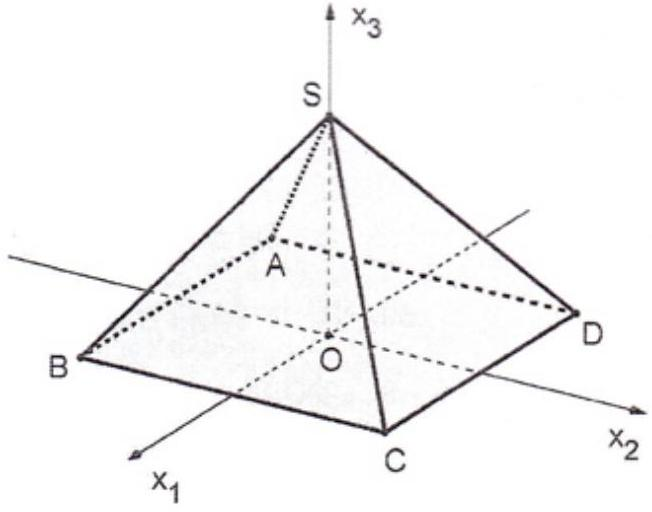
\includegraphics[max width=\textwidth, center]{2025_04_24_14fc0cc9eb4925701156g-2}

Abb. 1\\
a) Berechnen Sie den Inhalt der Oberfläche der Pyramide.\\
b) Genau eine der folgenden Gleichungen (1) bis (3) beschreibt eine Symmetrieebene der Pyramide. Geben Sie diese Gleichung an und begründen Sie für eine der anderen Gleichungen, dass die durch sie beschriebene Ebene keine Symmetrieebene der Pyramide ist.\\
(1) $x_{1}-x_{3}=0$\\
(2) $x_{1}+x_{2}+x_{3}=4$\\
(3) $x_{1}+x_{2}=0$\\
c) Bestimmen Sie eine Gleichung von E in Koordinatenform.\\
(zur Kontrolle: $4 \mathrm{x}_{2}+3 \mathrm{x}_{3}=12$ )\\
d) Es gibt einen Punkt $\mathrm{P}(0|0| p)$, der im Innern der Pyramide liegt und von allen vier Seitenflächen sowie der Grundfläche der Pyramide den gleichen Abstand hat. Mithilfe des folgenden Gleichungssystems lässt sich der Wert von $p$ bestimmen:\\
(I) $\overrightarrow{\mathrm{OQ}}=\left(\begin{array}{l}0 \\ 0 \\ \mathrm{p}\end{array}\right)+\mathrm{t} \cdot\left(\begin{array}{l}0 \\ 4 \\ 3\end{array}\right)$\\
(II) $4 \cdot 4 t+3 \cdot(p+3 t)=12$\\
(III) $|\overrightarrow{\mathrm{PQ}}|=\mathrm{p}$

Erläutern Sie die Überlegungen im geometrischen Zusammenhang, die diesem Vorgehen zur Bestimmung des Werts von p zugrunde liegen.\\
(5 BE)

Die Ebene $E$ gehört zur Schar der Ebenen $E_{k}: 4 k \cdot x_{1}+4 \sqrt{1-k^{2}} \cdot x_{2}+3 x_{3}=12$ mit $k \in[-1 ; 1]$. Die Seitenfläche ADS der Pyramide liegt in der Ebene $E_{-1}$ der Schar, die Seitenfläche BCS in der Ebene $\mathrm{E}_{1}$.\\
e) Zeigen Sie, dass der Punkt S in allen Ebenen der Schar enthalten ist. (1 BE)\\
f) Weisen Sie nach, dass die Größe des Winkels, unter dem die Gerade OS die Ebene $\mathrm{E}_{\mathrm{k}}$ schneidet, unabhängig von k ist.\\
(4 BE)\\
Jede Ebene $E_{k}$ der Schar schneidet die $x_{1} x_{2}$-Ebene in einer Gerade $g_{k}$. Mit $R_{k}$ wird jeweils derjenige Punkt auf $g_{k}$ bezeichnet, der von $O$ den kleinsten Abstand hat. In Abbildung 2 sind $g_{k}$ und $R_{k}$ beispielhaft für eine Ebene $E_{k}$ der Schar dargestellt.\\
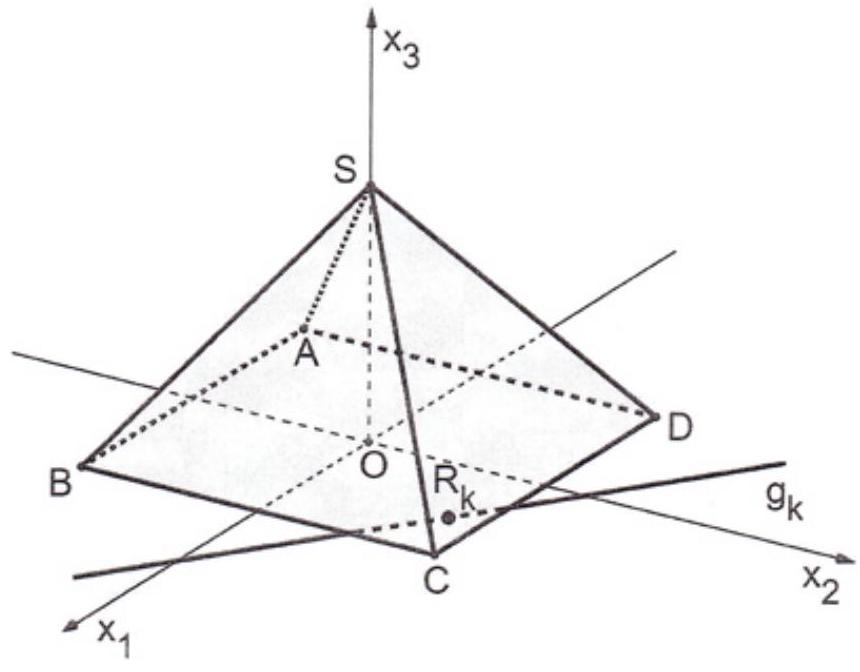
\includegraphics[max width=\textwidth, center]{2025_04_24_14fc0cc9eb4925701156g-3}

Abb. 2\\
g) Zeichnen Sie die Punkte $\mathrm{R}_{-1}$ und $\mathrm{R}_{1}$ in Abbildung 2 ein.\\
h) Durchläuft $k$ alle Werte von -1 bis 1, dann dreht sich die Fläche $\mathrm{OR}_{\mathrm{k}} \mathrm{S}$ um die Strecke $\overline{\text { OS }}$. Dabei entsteht ein Körper. Beschreiben Sie die Form des entstehenden Körpers und bestimmen Sie das Volumen dieses Körpers.

\section*{Lösungen}
\section*{Aufgabe II 1}
a) Flächeninhalt des Dreiecks CDS:

Länge der Grundseite: $\overline{\mathrm{CD}}=6 \mathrm{LE}$\\
Mittelpunkt der Strecke $\overline{\mathrm{CD}}$ ist $\mathrm{M}(0|3| 0)$.\\
Höhe des Dreiecks CDS: $h=\overrightarrow{M S}=|\overrightarrow{M S}|=\left|\left(\begin{array}{c}0 \\ -3 \\ 4\end{array}\right)\right|=\sqrt{9+16}=5 \mathrm{LE}$\\
Flächeninhalt des Dreiecks: $A=\frac{1}{2} \cdot \overline{\mathrm{CD}} \cdot \mathrm{h}=\frac{1}{2} \cdot 6 \cdot 5=15$\\
Oberfläche der Pyramide: $\mathrm{O}=\mathrm{A}_{\text {Grundfïche }}+4 \cdot 15=6 \cdot 6+60=96 \mathrm{FE}$\\
b) Eine Symmetrieebene der Pyramide muss die $\mathrm{x}_{3}$-Achse enthalten.

Das heißt, dass die Variable $\mathrm{x}_{3}$ nicht in der Koordinatengleichung vorkommen darf und das Ergebnis der Koordinatengleichung 0 sein muss. Damit muss es Gleichung (3) sein.

Gleichung (1) ist beispielsweise nicht möglich, weil die Symmetrieebene den Punkt S enthalten muss und die Koordinaten von S nicht die Gleichung (1) erfüllen.\\
c) Parameterform der Ebene $\mathrm{E}: \overrightarrow{\mathrm{x}}=\overrightarrow{\mathrm{OC}}+\mathrm{r} \cdot \overrightarrow{\mathrm{CD}}+\mathrm{s} \cdot \overrightarrow{\mathrm{CS}}=\left(\begin{array}{l}3 \\ 3 \\ 0\end{array}\right)+\mathrm{r} \cdot\left(\begin{array}{c}-6 \\ 0 \\ 0\end{array}\right)+\mathrm{s} \cdot\left(\begin{array}{c}-3 \\ -3 \\ 4\end{array}\right)$

Normalenvektor: $\overrightarrow{\mathrm{n}}=\left(\begin{array}{c}-6 \\ 0 \\ 0\end{array}\right) \times\left(\begin{array}{c}-3 \\ -.3 \\ 4\end{array}\right)=\left(\begin{array}{c}0 \\ 24 \\ 18\end{array}\right)$ bzw. $\overrightarrow{\mathrm{n}^{*}}=\left(\begin{array}{l}0 \\ 4 \\ 3\end{array}\right)$\\
$E: 4 x_{2}+3 x_{3}=d$\\
Einsetzen von $C(3|3| 0): 12+0=d \Leftrightarrow d=12$\\
Koordinatenform von $\mathrm{E}: 4 \mathrm{x}_{2}+3 \mathrm{x}_{3}=12$\\
d) I: Die Gleichung entspricht der Lotgeraden zur Ebene E (Richtungsvektor ist der Normalenvektor von E) durch den Punkt P. Der Punkt Q liegt auf dieser Lotgeraden.

II: Hier wird der Schnittpunkt der Lotgeraden mit der Ebene E berechnet. Der Punkt Q ist daher der Schnittpunkt von E mit der Lotgeraden.

III: Der Abstand von P zum Punkt Q (und damit der Abstand von P zur Ebene E) stimmt mit dem Abstand von $P$ zur Grundfläche überein.\\
Hinweis: Da die $x_{3}$-Koordinate von $P$ gleich $p$ ist, ist $p$ der Abstand von $P$ zur Grundfläche (also zur $\mathrm{x}_{1}-\mathrm{x}_{2}$-Ebene).\\
e) Einsetzen von $\mathrm{S}(0|0| 4)$ in die Ebenenschar:\\
$4 k \cdot 0+4 \cdot \sqrt{1-k^{2}} \cdot 0+3 \cdot 4=12 \Leftrightarrow 12=12$\\
Da die Aussage wahr ist unabhängig von $k$, liegt $S$ auf allen Ebenen der Schar.\\
f) Schnittwinkel der Ebene E mit der Gerade OS mit dem Richtungsvektor $\left(\begin{array}{l}0 \\ 0 \\ 4\end{array}\right)$.\\
$\sin (\alpha)=\frac{\left|\left(\begin{array}{c}4 k \\ 4 \sqrt{1-k^{2}} \\ 3\end{array}\right) \cdot\left(\begin{array}{l}0 \\ 0 \\ 4\end{array}\right)\right|}{\sqrt{16 \mathrm{k}^{2}+16\left(1-\mathrm{k}^{2}\right)+9} \cdot \sqrt{16}}=\frac{12}{\sqrt{16+9} \cdot 4}=\frac{3}{5}$\\
Da das Ergebnis unabhängig von $k$ ist, ist die Größe des Winkels unabhängig von k.\\
g) Die Ebene $\mathrm{E}_{-1}$ entspricht laut Aufgabenstellung der Ebene durch die Punkte ADS.

Die Gerade $\mathrm{g}_{-1}$ ist die Gerade durch die Punkte A und D.\\
Der Punkt $\mathrm{R}_{-1}(-3|0| 0)$ ist der Punkt auf $\mathrm{g}_{-1}$ mit dem kleinsten Abstand zu O(이이O).

Die Ebene $\mathrm{E}_{1}$ entspricht laut Aufgabenstellung der Ebene durch die Punkte BCS.\\
Die Gerade $\mathrm{g}_{1}$ ist die Gerade durch die Punkte B und C .\\
Der Punkt $\mathrm{R}_{1}(3|0| 0)$ ist der Punkt auf $\mathrm{g}_{1}$ mit dem kleinsten Abstand $\mathrm{zu} \mathrm{O}(0|0| 0)$.\\
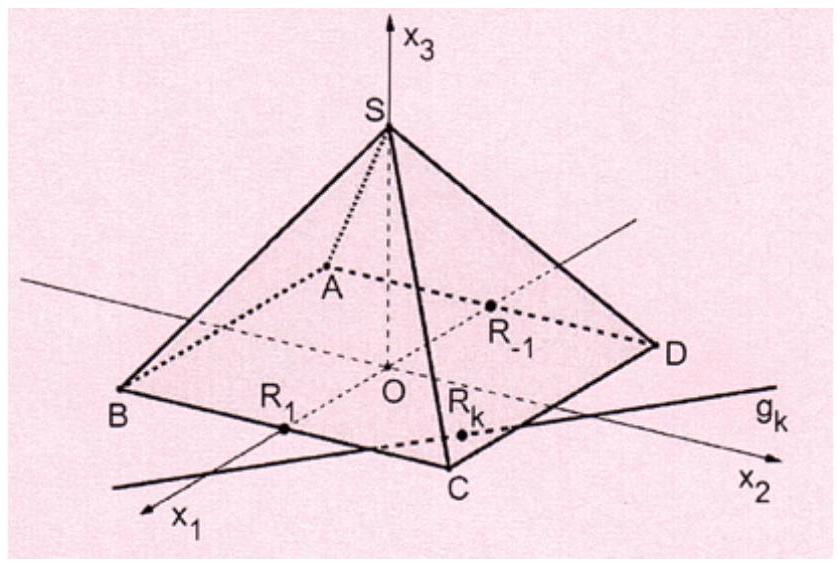
\includegraphics[max width=\textwidth, center]{2025_04_24_14fc0cc9eb4925701156g-5}\\
h) Der Körper ist ein halber Kegel mit der Spitze S.

Begründung:\\
Die Grundfläche besteht aus den Punkten $R_{k}$.\\
Der Abstand der Punkte $R_{k}$ vom Ursprung sind alle gleich groß, weil laut f) der Winkel zwischen der Ebenenschar und OS konstant und unabhängig von k ist.

Die eingezeichneten Randpunkte $\mathrm{R}_{-1}$ und $\mathrm{R}_{1}$ der Halbkreisfläche haben den Abstand 3 vom Ursprung, daher ist der Kegelradius $r=3$.\\
Die Höhe des Halbkegels ist $\mathrm{h}=\overline{\mathrm{OS}}=4$\\
$\mathrm{V}_{\text {Halbkegel }}=\frac{1}{2} \cdot \frac{1}{3} \cdot \pi \cdot \mathrm{r}^{2} \cdot \mathrm{~h}=\frac{1}{6} \cdot \pi \cdot 3^{2} \cdot 4=6 \pi$


\end{document}